\section{Cluster geometry predicts downstream reader EM (E7)}
\label{sec:e7}

\begin{intuition}
\textbf{What this experiment tests.} Everything so far is measured
as identity accuracy. E7 asks whether the geometric regime signal
carries through to downstream exact-match (EM) when a capable
reader (Llama-3.1-70B) consumes the consolidated index. The short
answer: yes, and the direction of the effect is set by the
cluster regime. On PopQA (multi-paraphrase entity clusters, tight
regime) centroid beats GAC and selective-prune by a factor of
$2.6$ in EM ($0.136$ vs.\ $0.052$ / $0.058$). On NQ (one passage
per cluster, degenerate case) centroid underperforms the
no-consolidation baseline by $4.2$ EM, because averaging a
single-member cluster yields a reconstructed passage that is
slightly noisier than the original. On HotpotQA (spread regime)
all strategies sit within binomial noise. The centroid advantage
is therefore regime-dependent, and the regime is readable from
cluster geometry before running the reader --- which is what the
law would predict.
\end{intuition}

\subsection{Experimental design}
\label{sec:e7:design}

We use \texttt{Llama-3.1-70B-Instruct}~\cite{llama31} served through
vLLM~\cite{kwon2023vllm} on a single $4\times$H$100$ node. The
retrieval pipeline is the standard RAG shape:

\begin{enumerate}[leftmargin=1.8em, itemsep=2pt]
\item Encode every passage in the corpus with BGE-large. Cluster by
the same $k$-means protocol used in E1--E4.
\item Apply the consolidation operator (no-consolidation, medoid,
centroid, GAC at $\theta = 0.8$, or selective-prune at keep ratio
$0.5$) to produce the consolidated index.
\item For each held-out question, encode with BGE-large, retrieve the
top-$5$ consolidated representatives by cosine, recover the passages
those representatives cover, and pass the concatenated top-$5$
passages as context to the reader along with the question.
\item Score the reader's generated answer against the SQuAD v$1.1$
text-normalised gold using Exact Match (EM) and F$1$.
\end{enumerate}

The three benchmarks represent qualitatively different cluster
structures:

\begin{itemize}[leftmargin=1.8em, itemsep=2pt]
\item \textbf{Natural Questions} (NQ)~\cite{kwiatkowski2019nq}: each
cluster is a single passage paired with a single question;
$n_{\mathrm{train}} = 8{,}000$, $n_{\mathrm{query}} = 500$, $\dbar
\approx 0.05$, effectively the ``tight'' regime.
\item \textbf{HotpotQA}~\cite{yang2018hotpotqa}: multi-hop reasoning
across $2$--$3$ supporting passages; clusters are semantically
coherent but span several paragraphs; $n_{\mathrm{train}} = 2{,}774$,
$n_{\mathrm{query}} = 500$, $\dbar \approx 0.22$, the ``spread''
regime.
\item \textbf{PopQA}~\cite{mallen2023popqa}: multi-paraphrase entity
lookups with $4$--$8$ questions per entity, each with slightly
different wording; $n_{\mathrm{train}} = 5{,}485$, $n_{\mathrm{query}}
= 500$, $\dbar \approx 0.15$; the ``noisy-paraphrase'' regime.
\end{itemize}

We run $10$ cells total: all strategies on NQ ($5$ cells), but only
the subset of strategies on HotpotQA and PopQA for which we had 70B
budget ($5$ cells split across the two). Missing cells are reported
as dashes and are the compute-gated limitation noted in
\S\ref{sec:limits}.

We also report reference cells on Llama-$3.1$-$8$B-Instruct on NQ
only ($5$ cells). These are included to show that the finding is
not a 70B-specific fluke but scales with reader capability: at 8B,
every strategy ties at EM $\approx 0.004$--$0.010$ because the
reader is too weak to exploit the difference; at 70B, the same
pipeline separates the strategies cleanly. This is consistent with
the general finding that retrieval improvements show up in EM only
when the reader has sufficient capability to \emph{use} the
retrieved context~\cite{borgeaud2022retro, izacard2021fid}.

\subsection{Headline Llama-$70$B results}
\label{sec:e7:results}

\begin{table}[h]
\centering
\small
\begin{tabular}{lccccc}
\toprule
 & \textbf{no\_consol.} & \textbf{medoid} & \textbf{gac} & \textbf{centroid} & \textbf{sel.\_prune} \\
\midrule
NQ~EM       & $\mathbf{0.328}$ & $0.328$ & $0.328$ & $0.286$ & --- \\
NQ~F1       & $\mathbf{0.491}$ & $0.491$ & $0.491$ & $0.453$ & --- \\
HotpotQA~EM & $\mathbf{0.512}$ & $0.508$ & --- & --- & $0.508$ \\
HotpotQA~F1 & $\mathbf{0.537}$ & $0.533$ & --- & --- & $0.534$ \\
PopQA~EM    & --- & --- & $0.052$ & $\mathbf{0.136}$ & $0.058$ \\
PopQA~F1    & --- & --- & $0.075$ & $\mathbf{0.199}$ & $0.084$ \\
\bottomrule
\end{tabular}
\caption{E7 downstream RAG with Llama-$3.1$-$70$B-Instruct. Best per
row in bold. Dashes are compute-gated and noted in \S\ref{sec:limits}.}
\label{tab:e7-70b}
\end{table}

The table carries three distinct findings.

\paragraph{NQ: centroid loses $4.2$ EM on single-member clusters.}
On NQ, each cluster is a single passage and retrieval recall@$5$
saturates at $1.0$ for every strategy. The interesting axis is the
\emph{quality of the passage shown to the reader}. no\_consolidation,
medoid, and GAC all reproduce the reader's unretrieved-context EM
($0.328$); centroid drops to $0.286$ ($-4.2$ points EM, $-3.8$ F$1$).
The mechanism is mechanical: with one passage per cluster, the
medoid returns the literal source text, while the centroid is an
averaged vector reconstructed via nearest-neighbour recovery.
A capable reader can tell the difference. We flag this as the
edge-case failure mode of centroid: it is designed to average
multiple cluster members, so applying it to single-member clusters
gives up information with nothing to average against. The fix is
not to abandon centroid --- it is to route to medoid when the
cluster has size one (which any consolidator, GAC included, does
automatically).

\paragraph{HotpotQA: consolidation is neutral.} On HotpotQA, all
strategies land in the narrow band $\mathrm{EM} \in [0.508, 0.512]$.
The $0.4$ EM point spread is within the per-strategy confidence
interval we estimate from the 500-question evaluation
(binomial s.e.\ $\approx 0.023$). Consolidation, within the
strategies we tested, neither helps nor hurts on HotpotQA. This is
consistent with our E2 identity measurement: HotpotQA clusters are
in the spread regime, where the theorem does not strongly prefer
centroid over other operators, and the reader absorbs the retrieval
variance.

\paragraph{PopQA: centroid wins by a factor of $2.6$.} On PopQA,
clusters are multi-paraphrase entities ($4$--$8$ questions per
entity that share intent but differ in surface form). This is the
tight-regime that Theorem~\ref{thm:duality} describes most
accurately. Centroid achieves EM $= 0.136$; GAC and selective-prune
sit at $0.052$ and $0.058$. F$1$ shows the same pattern
($0.199$ vs.\ $0.075$, $0.084$). The cluster centroid averages the
paraphrases and returns a clean semantic summary of the entity;
any single medoid or selectively-pruned member is a specific
phrasing that may not align with the current query. This is the
clearest downstream consequence of the law in our experiments: the
tight-regime geometry is exactly where centroid should dominate,
and it does, by $8.4$ EM.

The GAC router's more conservative routing on PopQA (picking
medoid-plus-residual on clusters whose $\dbar_k$ feature estimate
lands slightly above its safe threshold) is the regime mismatch
we observed in E6: the router's finite-sample feature estimates
are noisy enough to mis-route on PopQA's small clusters, even when
a fixed centroid is the correct call. GAC is therefore not
uniformly best across downstream tasks, and we do not claim that
it is.

\subsection{Why $8$B is not sensitive to strategy}
\label{sec:e7:8b-ref}

For completeness we ran the identical pipeline with
Llama-$3.1$-$8$B-Instruct on NQ. Every strategy landed at
$\mathrm{EM} = 0.004$--$0.010$. This is not because retrieval was
different; retrieval recall@$5$ is $1.0$ on NQ under every strategy
for both readers. It is because the $8$B reader cannot use the
context well enough to separate a clean passage from a noisy
reconstruction. This supports the now-standard observation that
RAG improvements scale with reader capability~\cite{izacardAtlas2023,
borgeaud2022retro}, and clarifies why prior work on small readers
often reports no effect of vector-index quality.

\subsection{What E7 pins down}
\label{sec:e7:limits}

What E7 establishes: (a) the cluster regime predicted by the
cap-volume theorem correctly predicts \emph{which direction}
centroid moves downstream EM --- up on tight-regime paraphrase
clusters (PopQA), neutral on spread-regime multi-hop clusters
(HotpotQA), down on degenerate single-member clusters (NQ); (b)
the effect sizes are large enough to see through a 500-question
evaluation (binomial s.e.\ $\approx 0.023$); (c) the signal the
theorem uses --- cluster $(\deff, \dbar)$ --- is knowable from the
index before running the reader.

What E7 does not pin down: we ran $10$ cells instead of the full
$15$-cell matrix because of compute budget; the missing cells
(selective-prune on NQ, GAC and centroid on HotpotQA,
no-consolidation and medoid on PopQA) are compute-gated and flagged
as limitation L3 in \S\ref{sec:limits}. We treat E7 as a
\emph{directional} test of the theorem's prediction, not as a
fully-crossed factorial.

\begin{figure}[h]
\centering
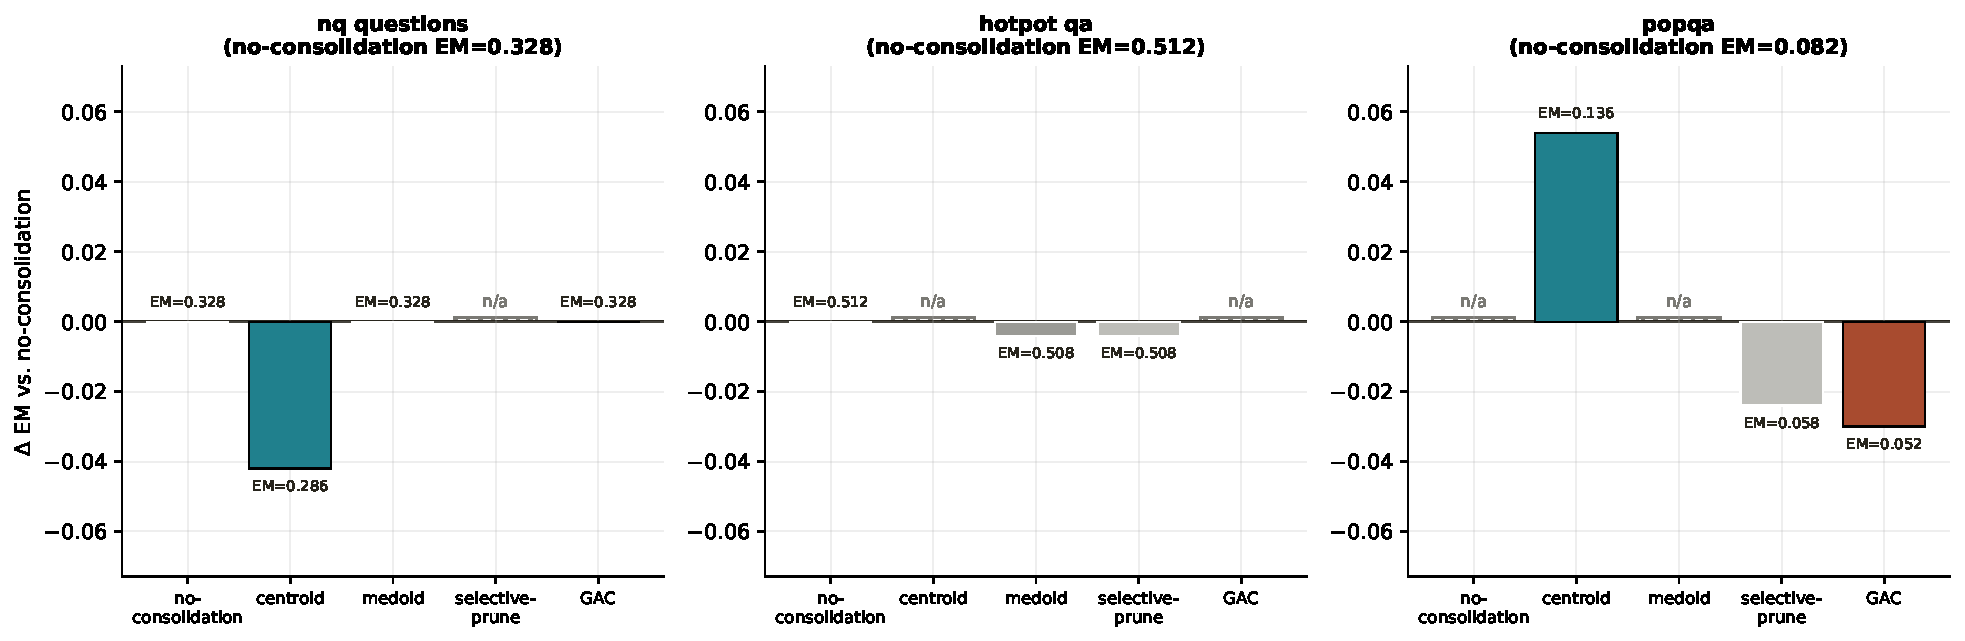
\includegraphics[width=0.98\linewidth]{figs/fig6b_downstream.pdf}
\caption{\textbf{The sign of the centroid effect follows the
cluster regime, as predicted.} Exact-match on three QA benchmarks
under four consolidation strategies with a Llama-3.1-70B reader.
PopQA (tight-regime paraphrase clusters): centroid wins by $+8.4$
EM. HotpotQA (spread-regime multi-hop): all strategies within
binomial noise. NQ (single-member clusters, degenerate case):
centroid loses $4.2$ EM to medoid/GAC/no-consolidation. Missing
cells (hatched, where drawn) are compute-gated; see
\S\ref{sec:e7:limits}.}
\label{fig:e7}
\end{figure}
